%label:"fig:hamiltonianOnSphere"
%author:JeffHicks
%name:"rotation of sphere"
%type:"figure"
%parent:exm:sphereRotation
%caption:"The Hamiltonian flow of the standard height function rotates the sphere counterclockwise relative to the north pole"

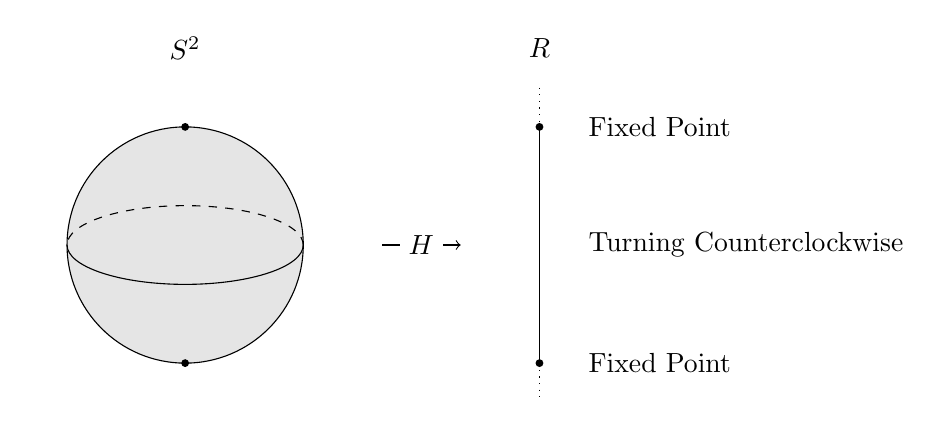
\begin{tikzpicture}
    \draw[fill=gray!20]  (-2,2) ellipse (1.5 and 1.5);
    \begin{scope}[]
    \clip  (-4,2) rectangle (0,3);
    \draw[dashed]  (-2,2) ellipse (1.5 and 0.5);
    \end{scope}
    \begin{scope}[]
    \clip  (-4,2) rectangle (0,1);
    \draw  (-2,2) ellipse (1.5 and 0.5);
    \end{scope}
    
    \draw (2.5,3.5) -- (2.5,0.5);
    \draw[->] (0.5,2) -- (1.5,2);
    \node[fill=white] at (1,2) {$H$};
    \draw[dotted] (2.5,4) -- (2.5,3.5) (2.5,0.5) -- (2.5,0);
    \node at (-2,4.5) {$S^2$};
    \node at (2.5,4.5) {$\mathbb R$};
    \node[right] at (3,3.5) {Fixed Point};
    \node[right] at (3,2) {Turning Counterclockwise};
    \node[right] at (3,0.5) {Fixed Point};
    \node[circle, fill=black, scale=.3] at (-2,3.5) {};
    \node[circle, fill=black, scale=.3] at (-2,0.5) {};
    \node[circle, fill=black, scale=.3] at (2.5,0.5) {};
    \node[circle, fill=black, scale=.3] at (2.5,3.5) {};
    \end{tikzpicture}